\documentclass[hidelinks,12pt]{article}
\usepackage[left=0.25cm,top=1cm,right=0.25cm,bottom=1cm]{geometry}
%\usepackage[landscape]{geometry}
\textwidth = 20cm
\hoffset = -1cm
\usepackage[utf8]{inputenc}
\usepackage[spanish,es-tabla]{babel}
\usepackage[autostyle,spanish=mexican]{csquotes}
\usepackage[tbtags]{amsmath}
\usepackage{nccmath}
\usepackage{amsthm}
\usepackage{amssymb}
\usepackage{mathrsfs}
\usepackage{graphicx}
\usepackage{subfig}
\usepackage{standalone}
\usepackage[outdir=./Imagenes/]{epstopdf}
\usepackage{siunitx}
\usepackage{physics}
\usepackage{color}
\usepackage{float}
\usepackage{hyperref}
\usepackage{multicol}
%\usepackage{milista}
\usepackage{anyfontsize}
\usepackage{anysize}
%\usepackage{enumerate}
\usepackage[shortlabels]{enumitem}
\usepackage{capt-of}
\usepackage{bm}
\usepackage{relsize}
\usepackage{placeins}
\usepackage{empheq}
\usepackage{cancel}
\usepackage{wrapfig}
\usepackage[flushleft]{threeparttable}
\usepackage{makecell}
\usepackage{fancyhdr}
\usepackage{tikz}
\usepackage{bigints}
\usepackage{scalerel}
\usepackage{pgfplots}
\usepackage{pdflscape}
\pgfplotsset{compat=1.16}
\spanishdecimal{.}
\renewcommand{\baselinestretch}{1.5} 
\renewcommand\labelenumii{\theenumi.{\arabic{enumii}})}
\newcommand{\ptilde}[1]{\ensuremath{{#1}^{\prime}}}
\newcommand{\stilde}[1]{\ensuremath{{#1}^{\prime \prime}}}
\newcommand{\ttilde}[1]{\ensuremath{{#1}^{\prime \prime \prime}}}
\newcommand{\ntilde}[2]{\ensuremath{{#1}^{(#2)}}}

\newtheorem{defi}{{\it Definición}}[section]
\newtheorem{teo}{{\it Teorema}}[section]
\newtheorem{ejemplo}{{\it Ejemplo}}[section]
\newtheorem{propiedad}{{\it Propiedad}}[section]
\newtheorem{lema}{{\it Lema}}[section]
\newtheorem{cor}{Corolario}
\newtheorem{ejer}{Ejercicio}[section]

\newlist{milista}{enumerate}{2}
\setlist[milista,1]{label=\arabic*)}
\setlist[milista,2]{label=\arabic{milistai}.\arabic*)}
\newlength{\depthofsumsign}
\setlength{\depthofsumsign}{\depthof{$\sum$}}
\newcommand{\nsum}[1][1.4]{% only for \displaystyle
    \mathop{%
        \raisebox
            {-#1\depthofsumsign+1\depthofsumsign}
            {\scalebox
                {#1}
                {$\displaystyle\sum$}%
            }
    }
}
\def\scaleint#1{\vcenter{\hbox{\scaleto[3ex]{\displaystyle\int}{#1}}}}
\def\bs{\mkern-12mu}


\title{La función delta de Dirac \\ \large {Matemáticas Avanzadas de la Física}\vspace{-3ex}}

\author{M. en C. Gustavo Contreras Mayén}
\date{ }

\pagestyle{fancy}
\fancyhf{}
\rhead{Curso MAF}
\lhead{\leftmark}
\rfoot{\thepage}
\setlength{\headheight}{16pt}%


\begin{document}
\maketitle
\fontsize{14}{14}\selectfont
\tableofcontents
\newpage

%Referencia Kusse - Chapter 5

\section{Introducción.}

La función $\delta$ de Dirac es una función extraña pero útil que tiene muchas aplicaciones en ciencia, ingeniería y matemáticas. 
\par
La función $\delta$ fue propuesta en 1930 por Paul Dirac en el desarrollo del formalismo matemático de la mecánica cuántica. Necesitaba una función que fuera cero en todas partes, excepto en un solo punto, donde era discontinua y se comportaba como un pico infinitamente alto e infinitamente estrecho de área unitaria.
\par
Los matemáticos se apresuraron a señalar que, estrictamente hablando, no hay ninguna función que tenga estas propiedades. Pero Dirac supuso que sí, y procedió a utilizarlo con tanto éxito que se desarrolló una nueva rama de las matemáticas para justificar su uso. Esta área de las matemáticas se denomina \emph{teoría de funciones generalizadas} y desarrolla, con todo detalle, la base de la función $\delta$ de Dirac. Este tratamiento riguroso es necesario para justificar el uso de estas funciones discontinuas, pero para el físico las interpretaciones físicas más simples son igualmente importantes.

\section{Funciones singulares en física.}

Las situaciones físicas se modelan generalmente mediante ecuaciones y operaciones sobre funciones continuas. A veces, sin embargo, es útil considerar idealizaciones discontinuas, como la densidad de masa de una masa puntual o la fuerza de un impulso mecánico infinitamente rápido.
\par
Las funciones que describen estas ideas son obviamente extremadamente discontinuas, porque ellas y todas sus derivadas deben divergir. Por esta razón, a menudo se les llama \emph{funciones singulares}. La función $\delta$ de Dirac se desarrolló para describir funciones que involucran este tipo de discontinuidades y proporcionar un método para manejarlas en ecuaciones que normalmente solo involucran funciones continuas.

\subsection{El impulso ideal.}

A menudo, el primer encuentro de un estudiante de física con la función $\delta$ es el impulso \enquote{ideal}.
\par
En mecánica, un impulso es una fuerza que actúa sobre un objeto durante un período de tiempo finito. Considera la fuerza realista representada en la figura (\ref{fig:f1}).

\begin{figure}[H]
\centering
\subfloat[]{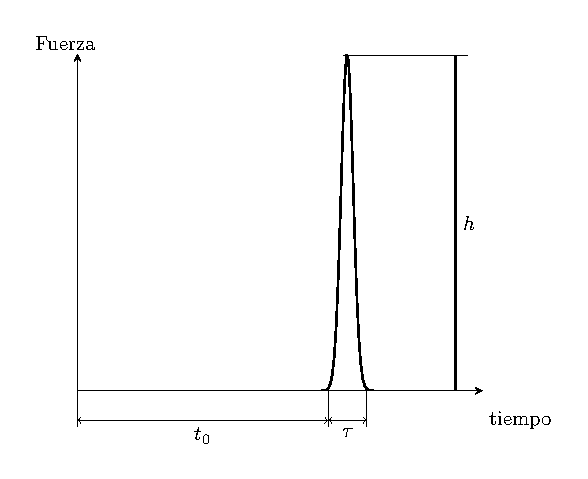
\includegraphics[width=0.5\textwidth]{Imagenes/delta_Dirac_01.eps}\label{fig:f1}}
\subfloat[]{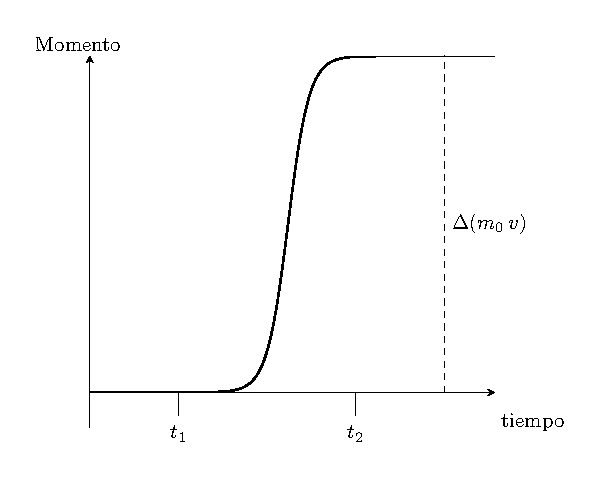
\includegraphics[width=0.5\textwidth]{Imagenes/delta_Dirac_Momento_01.eps}\label{fig:f2}}
\caption{Cambio en la fuerza y momento.}
\end{figure}

Vale cero hasta $t = t_{1}$, cuando aumenta suavemente desde cero hasta su valor máximo, y luego finalmente regresa a cero en $t = t_{2}$. Cuando esta fuerza se aplica a un objeto de masa $m_{0}$, el momento en la dirección de la fuerza aplicada cambia, como se muestra en la figura (\ref{fig:f2}). La cantidad de movimiento permanece constante hasta $t = t_{1}$, cuando comienza a cambiar continuamente hasta alcanzar su valor final en $t = t_{2}$.

\end{document}